\clearpage
\section{System Overview}
\subsection{System Block Diagram}
\begin{figure}[h]
    \centering
    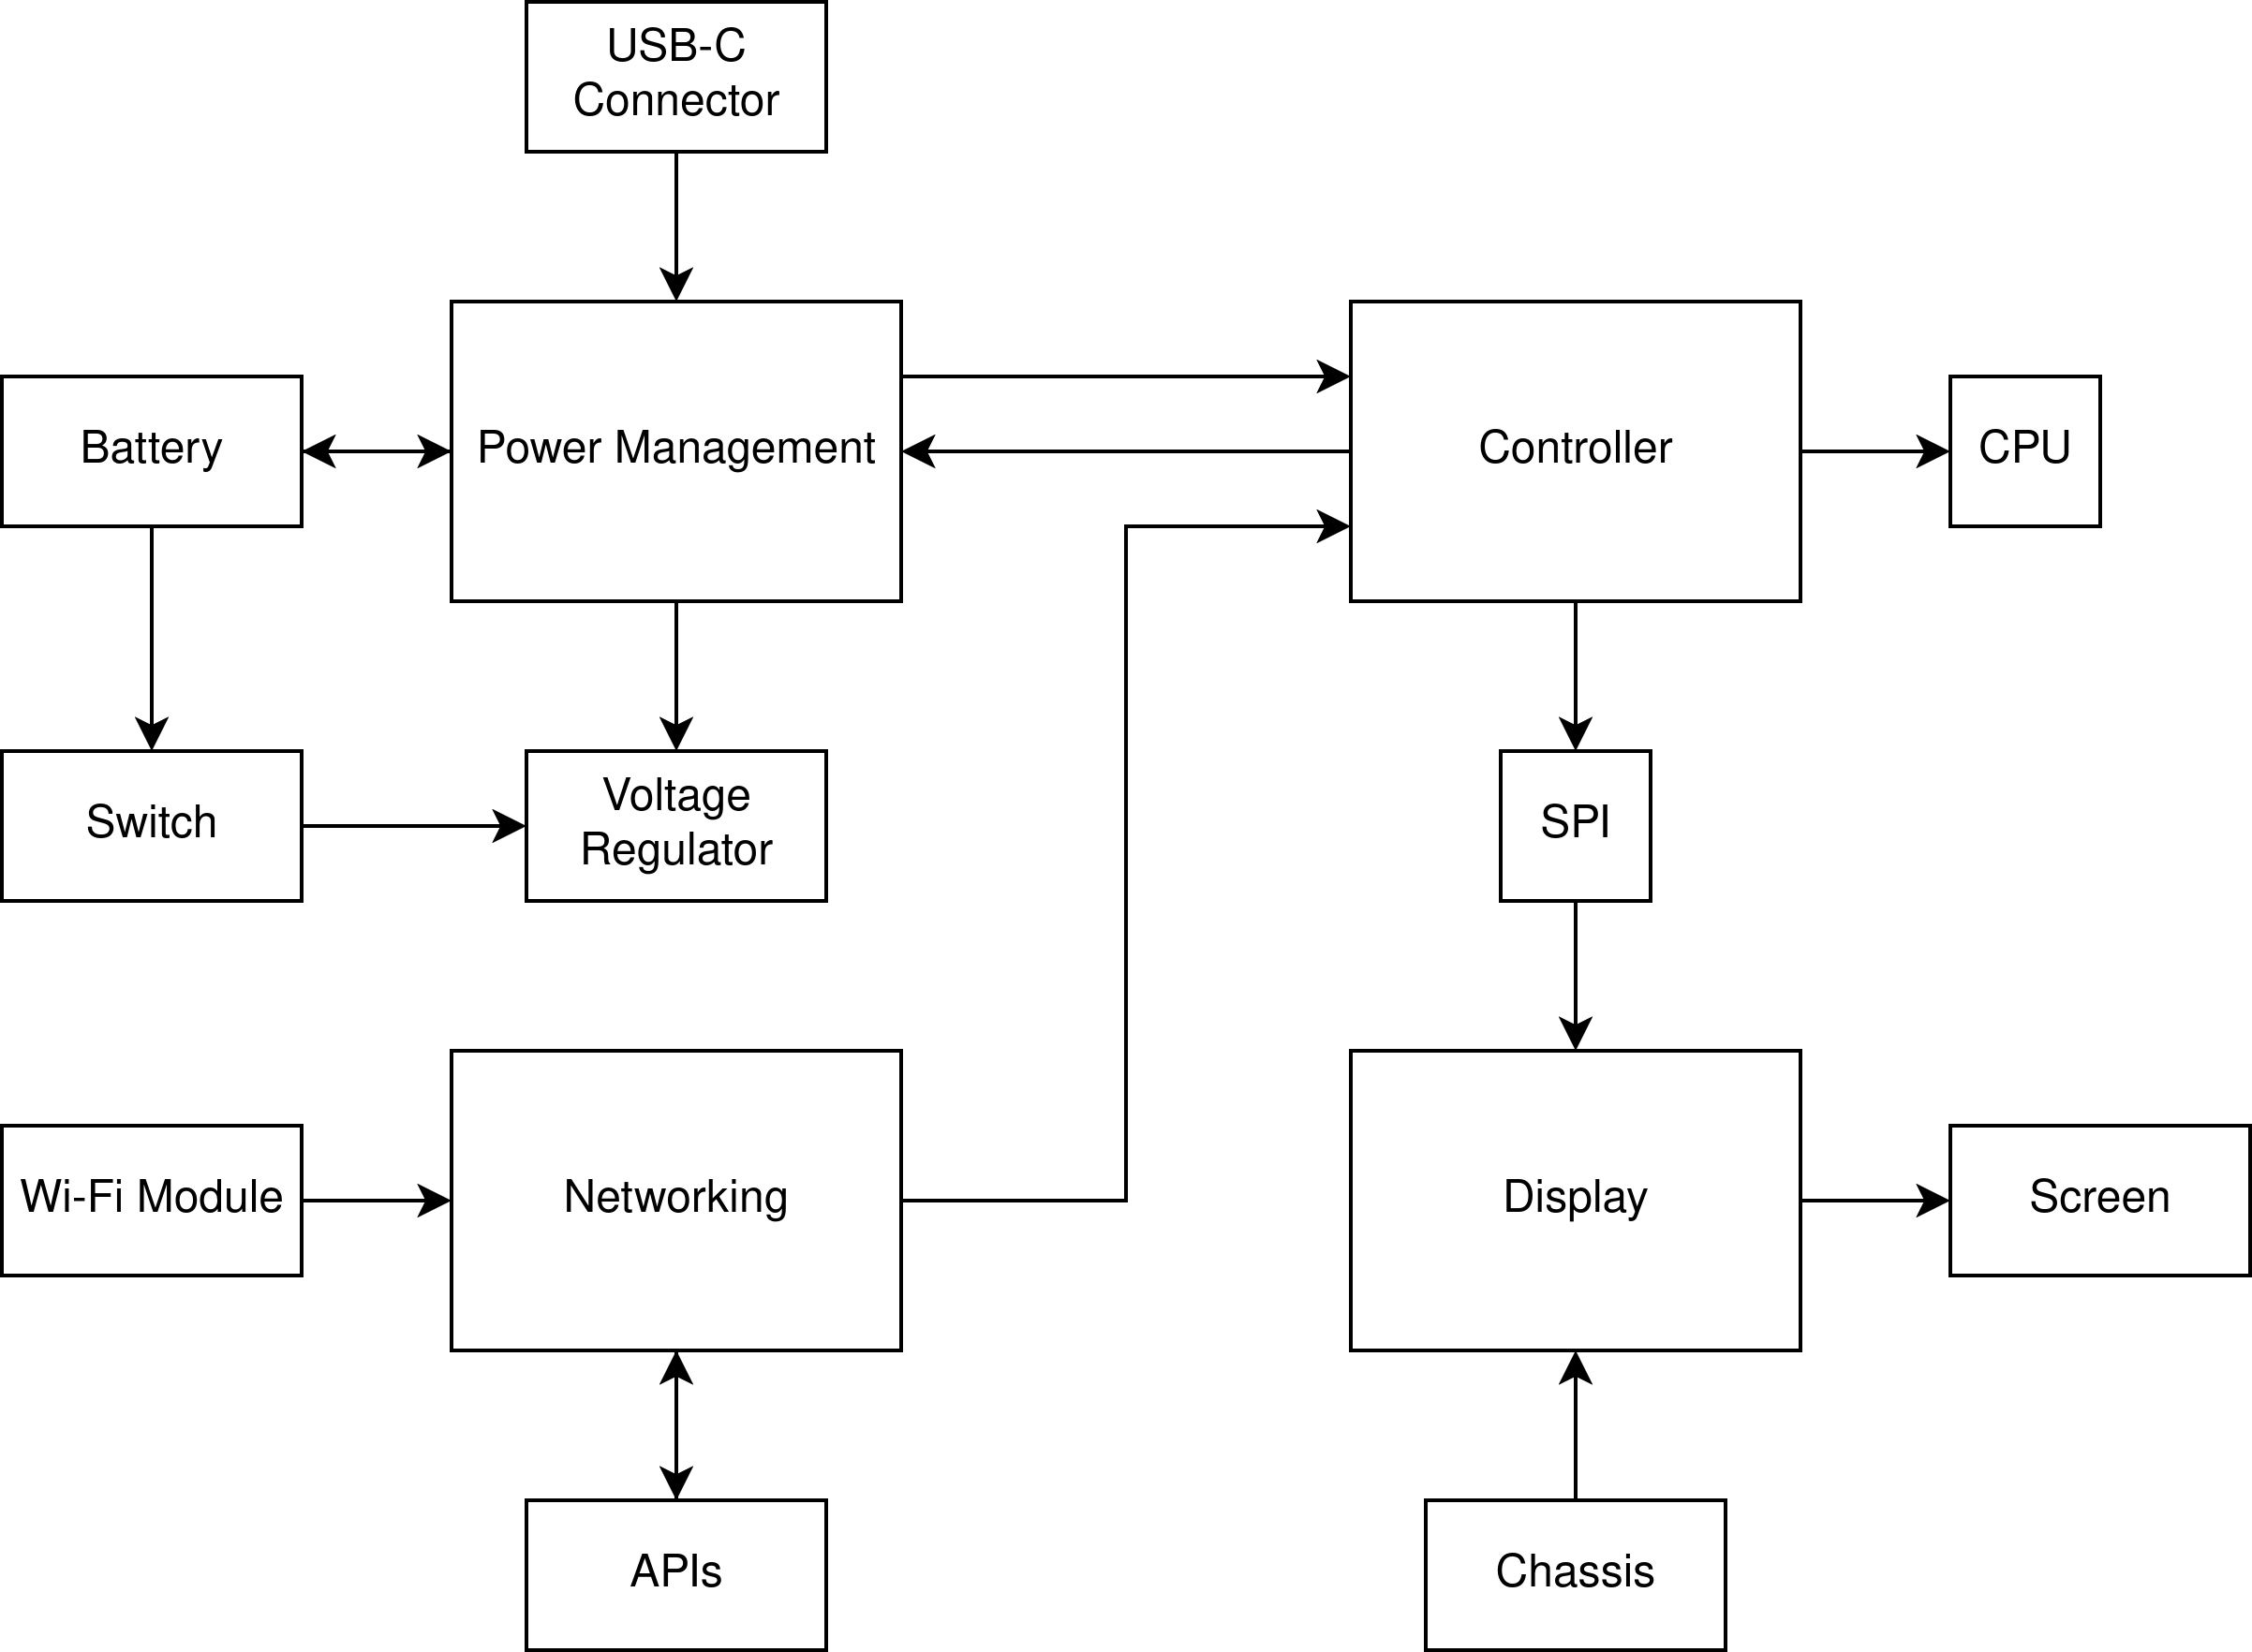
\includegraphics[width=16cm]{images/block_diagram.png}
    \caption{System Block Diagram}
\end{figure}

% Activity Diagram
\clearpage
\subsection{System Activity Diagram}
\begin{figure}[h]
    \centering
    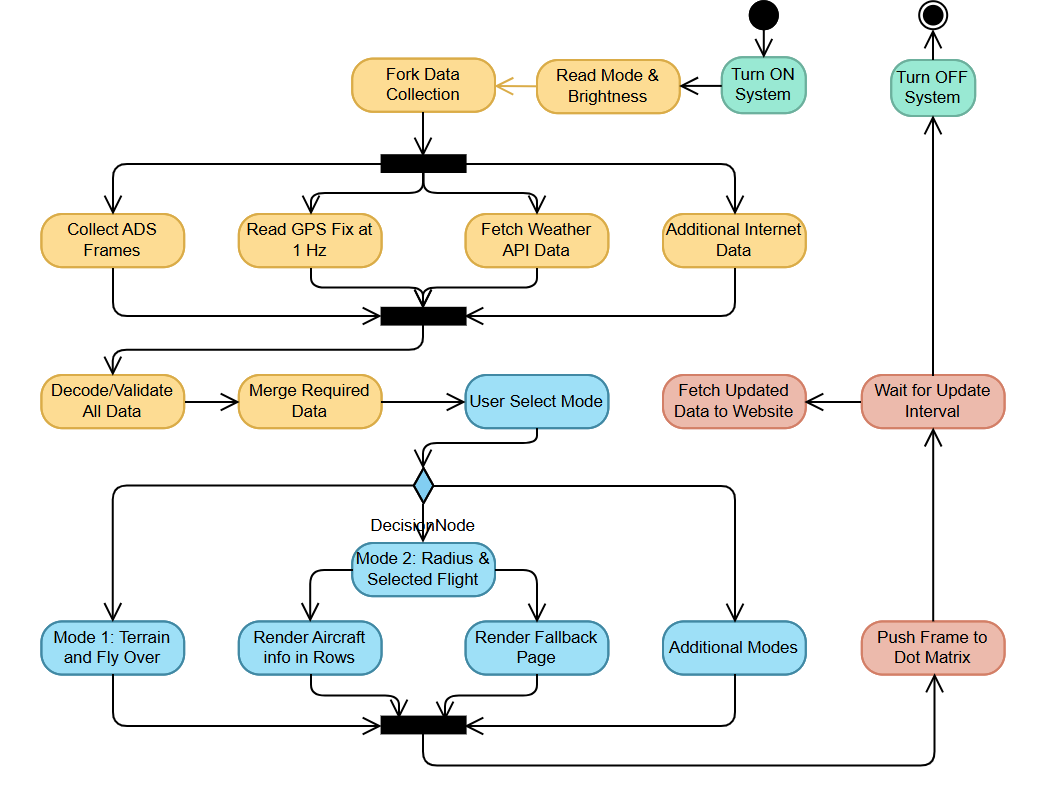
\includegraphics[width=16cm]{images/systemactivitydiagram.png} % Change the picture
    \caption{System Activity Diagram}
\end{figure}

% Mechanical Design
\clearpage
\subsection{System Mechanical Design (Extra Credit)}
[\textbf{DD3+}]
\begin{figure}[h]
    \centering
    
\includegraphics[width=16cm]{images/white.png} % Change the picture
    \caption{System Mechanical Design}
\end{figure}

% Integration Approach
\clearpage
\subsection{Integration Approach}
[\textbf{DD3+}]
[Theory behind the system design, with reference to subsystem integration within your system – i.e., explain how it is supposed to work, but not whether it did actually work]
[Type here]

% System Photograph
\clearpage
\subsection{System Photographs} % Have as many photoes as you need
[\textbf{DD3+}]
[Photograph of assembled system, intended to highlight user interaction / controls. If system is split into multiple parts, show a composite of more than one photograph with all key user interactions / controls. ]
\begin{figure}[h]
    \centering
    
\includegraphics[width=16cm]{images/white.png} % Change the picture
    \caption{[Photo Name]}
\end{figure}